\section{Exercise G}
We have to show that $ \forall x (P(x) \to \exists y K(x,y)) $ is logically equivalent to $ \forall x \exists y (P(x) \to K(x,y)) $, thus:
\[ \forall x (P(x) \to \exists y K(x,y)) \equiv \forall x \exists y (P(x) \to K(x,y)) \]
Using the tableau method we can analyze the equivalent formula:
\[ \forall x (P(x) \to \exists y K(x,y)) \leftrightarrow \forall x \exists y (P(x) \to K(x,y)) \]
Tableau method on next page.
\newpage

\begin{center}
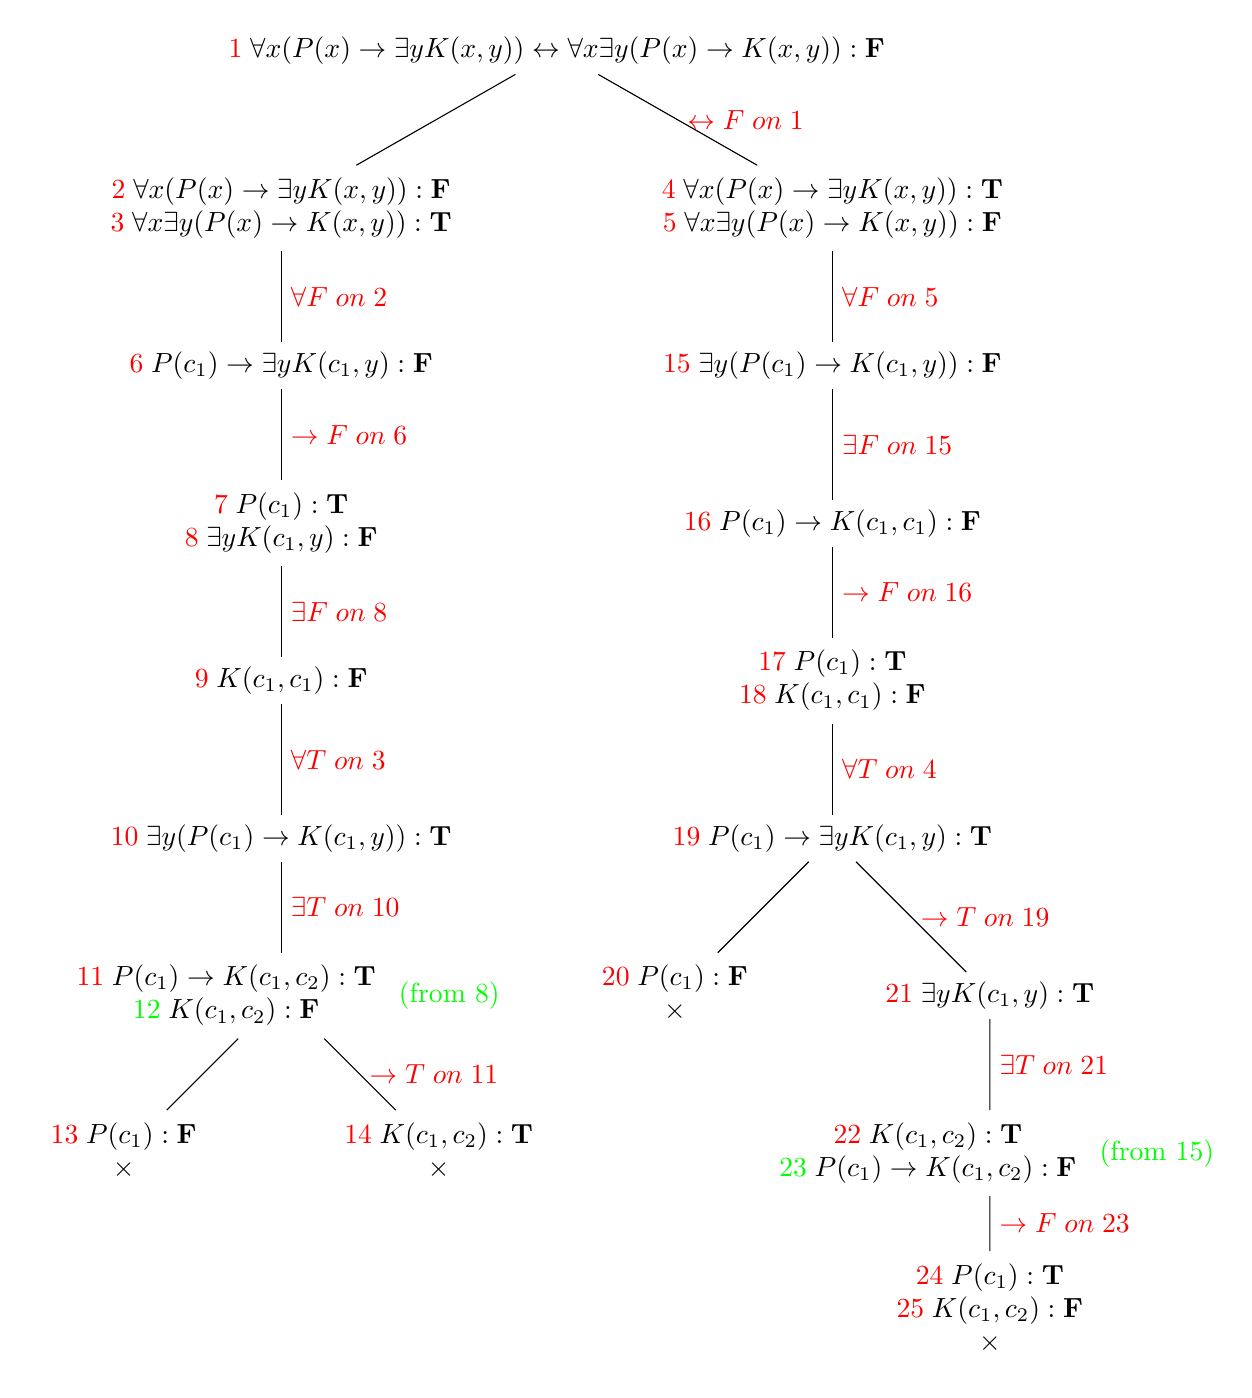
\begin{tikzpicture}
\node {$ \textcolor{red}{1}\; \forall x (P(x) \to \exists y K(x,y)) \leftrightarrow \forall x \exists y (P(x) \to K(x,y)):\textbf{F} $} [sibling distance = 7cm] [level distance=20mm] 
        child {node {$ \begin{array}{c} \textcolor{red}{2}\; \forall x (P(x) \to \exists y K(x,y)):\textbf{F} \\  \textcolor{red}{3}\; \forall x \exists y (P(x) \to K(x,y)):\textbf{T} \end{array} $}
                child {node {$ \textcolor{red}{6}\; P(c_1) \to \exists y K(c_1,y):\textbf{F} $}
                    child {node {$ \begin{array}{c} \textcolor{red}{7}\; P(c_1):\textbf{T} \\ \textcolor{red}{8}\; \exists y K(c_1,y):\textbf{F} \end{array} $}
                         child {node {$ \textcolor{red}{9}\; K(c_1,c_1):\textbf{F} $}
                            child {node {$ \textcolor{red}{10}\; \exists y (P(c_1) \to  K(c_1,y)):\textbf{T} $}
                                child {node {$ \begin{array}{c} \textcolor{red}{11}\; P(c_1) \to  K(c_1,c_2):\textbf{T} \\ \textcolor{green}{12}\; K(c_1,c_2):\textbf{F} \end{array} $ \textcolor{green}{(from 8)}} [sibling distance = 4cm]
                                    child {node {$ \begin{array}{c} \textcolor{red}{13}\; P(c_1):\textbf{F} \\ \times \end{array} $}}
                                    child {node {$ \begin{array}{c} \textcolor{red}{14}\; K(c_1,c_2):\textbf{T} \\ \times \end{array} $}
                                        edge from parent node [right, red] {$\to T\;on\; 11$}}
                                        edge from parent node [right, red] {$\exists T\;on\; 10$}} 
                                        edge from parent node [right, red] {$\forall T\;on\; 3$}}         
                                        edge from parent node [right, red] {$\exists F\;on\; 8$}}
                                        edge from parent node [right, red] {$\to F\;on\; 6$}}
                                        edge from parent node [right, red] {$\forall F\;on\; 2$}}}
        child {node {$ \begin{array}{c} \textcolor{red}{4}\; \forall x (P(x) \to \exists y K(x,y)):\textbf{T} \\  \textcolor{red}{5}\; \forall x \exists y (P(x) \to K(x,y)):\textbf{F} \end{array} $} [level distance=20mm]
            child {node {$ \textcolor{red}{15}\; \exists y (P(c_1) \to K(c_1,y)):\textbf{F} $}
                 child {node {$ \textcolor{red}{16}\; P(c_1) \to K(c_1,c_1):\textbf{F} $}
                    child {node {$ \begin{array}{c} \textcolor{red}{17}\; P(c_1):\textbf{T} \\ \textcolor{red}{18}\; K(c_1,c_1):\textbf{F} \end{array} $}
                        child {node {$ \textcolor{red}{19}\; P(c_1) \to \exists y K(c_1,y):\textbf{T} $} [sibling distance = 4cm]
                            child {node {$ \begin{array}{c} \textcolor{red}{20}\; P(c_1):\textbf{F} \\ \times \end{array} $}}
                            child {node {$ \textcolor{red}{21}\; \exists y K(c_1,y):\textbf{T} $}
                                child {node {$ \begin{array}{c} \textcolor{red}{22}\; K(c_1,c_2):\textbf{T} \\ \textcolor{green}{23}\; P(c_1) \to K(c_1,c_2):\textbf{F} \end{array} $ \textcolor{green}{(from 15)}}
                                    child {node {$ \begin{array}{c} \textcolor{red}{24}\; P(c_1):\textbf{T} \\ \textcolor{red}{25}\; K(c_1,c_2):\textbf{F} \\ \times \end{array} $}
                                    edge from parent node [right, red] {$\to F\;on\; 23$}}
                                    edge from parent node [right, red] {$\exists T\;on\; 21$}}
                                    edge from parent node [right, red] {$\to T\;on\; 19$}}
                                    edge from parent node [right, red] {$\forall T\;on\; 4$}}
                                    edge from parent node [right, red] {$\to F\;on\; 16$}}
                                    edge from parent node [right, red] {$\exists F\;on\; 15$}}
                                    edge from parent node [right, red] {$\forall F\;on\; 5$}}
                                    edge from parent node [right, red] {$\leftrightarrow F\;on\; 1$}};
\end{tikzpicture}
\end{center}
\noindent
As can be seen, all branches of the tableau closes, and for that reason there is no falsifying assignment for the statement. Hence, the statement is valid, and as such, the two formulae are equivalent.